\documentclass[12pt,a4paper]{article}
\usepackage{graphicx}
\usepackage{geometry}
\usepackage{hyperref}
\usepackage{amsmath}
\usepa\begin{figure}[H]
    \centering
    \includegraphics[width=0.7\textwidth]{images/DeploymentDiagram.png}
    \caption{Deployment diagram of the greenhouse system}
    \label{fig:deployment}
\end{figure}float}
\geometry{margin=1in}
\title{Design and Implementation of a Smart Greenhouse Automation System Using CoAP and ESP32}
\author{Azamkhon Khudoyberdiev}
\date{\today}

\begin{document}

\maketitle
\newpage
\tableofcontents
% Remove unwanted preamble content and set up page numbering
% No page numbers for title and TOC
\pagenumbering{gobble}
\maketitle
\newpage
% Start page numbering (arabic) from Introduction
\pagenumbering{arabic}

\section*{Abstract}
\addcontentsline{toc}{section}{Abstract}
This report presents the design, implementation, and evaluation of a smart greenhouse automation system leveraging IoT technologies. The system integrates distributed wireless sensor nodes, automated irrigation, and real-time data analytics to optimize resource usage and improve crop health. Experimental results and case studies demonstrate significant improvements in water efficiency, crop yield, and labor reduction, highlighting the system’s potential for sustainable agriculture in Uzbekistan and similar regions.

\cite{FAO2017,SmartAgReview,ESP32Survey,CoAPRFC,Netafim2020,Priva2021,IoTGreenhouse2022}


\section{Introduction}
Greenhouse farming enables controlled cultivation of plants, but traditional methods often result in inefficient resource use and inconsistent crop quality. This report proposes a comprehensive IoT-based solution to address these challenges, focusing on the integration of sensors, microcontrollers, and server technologies for optimal plant growth and resource management. The system is evaluated through both simulation and real-world deployment.

Recent studies highlight the importance of IoT in agriculture for improving efficiency and sustainability~\cite{SmartAgReview,IoTGreenhouse2022}.


\section{Background and Motivation}
With global food demand projected to rise by 70\% by 2050 (FAO), sustainable agriculture is critical. Conventional irrigation methods can waste up to 60\% of water. Smart greenhouses, by contrast, can reduce water usage by up to 30\% and increase yields by 20\%. This project aims to demonstrate these benefits using modern IoT components and protocols.

The Food and Agriculture Organization (FAO) projects a significant increase in food demand~\cite{FAO2017}. Smart greenhouse systems have been shown to reduce water usage and increase yields~\cite{IoTGreenhouse2022,SmartAgReview}.


\section{Market Overview}
The smart agriculture market is rapidly expanding, with leading companies such as Autogrow, Priva, Netafim, Growlink and Artemis offering solutions ranging from sensor hardware to cloud-based analytics. These platforms exemplify the state-of-the-art in greenhouse automation and data-driven farming.

For example, Netafim and Priva are recognized for their advanced irrigation and climate control solutions~\cite{Netafim2020,Priva2021}.


\section{System Architecture}
The proposed system consists of distributed sensor nodes, Wi-Fi routers, and a central server. Each node monitors environmental parameters and controls irrigation, while the server aggregates data, manages automation, and provides remote access via a secure internet connection.

The use of ESP32 microcontrollers and wireless protocols is common in modern IoT deployments~\cite{ESP32Survey}.

\subsection{Key Challenges}
\begin{itemize}
    \item Maintaining optimal temperature and humidity
    \item Preventing over- or under-watering
    \item Early detection of plant diseases
    \item Reducing manual labor
    \item Ensuring data security and system reliability
\end{itemize}


\subsection{Node Design}
Each plant is equipped with a sensor node comprising:
\begin{itemize}
    \item Humidity (DHT22), Temperature (DS18B20), Light (BH1750), Pressure (BMP280), Soil Moisture (Capacitive), and Soil EC (Analog EC) sensors
    \item ESP32 microcontroller with Wi-Fi antenna
    \item Li-Ion battery (18650, 2600mAh)
    \item Camera (OV2640)
    \item Solenoid valve (bi-phased, 12V)
\end{itemize}
The solenoid is controlled by the MCU, which communicates with the main server using the CoAP protocol. The server can remotely trigger irrigation as needed.

CoAP is widely used for resource-constrained IoT devices due to its lightweight nature~\cite{CoAPRFC}.

\begin{figure}[H]
    \centering
    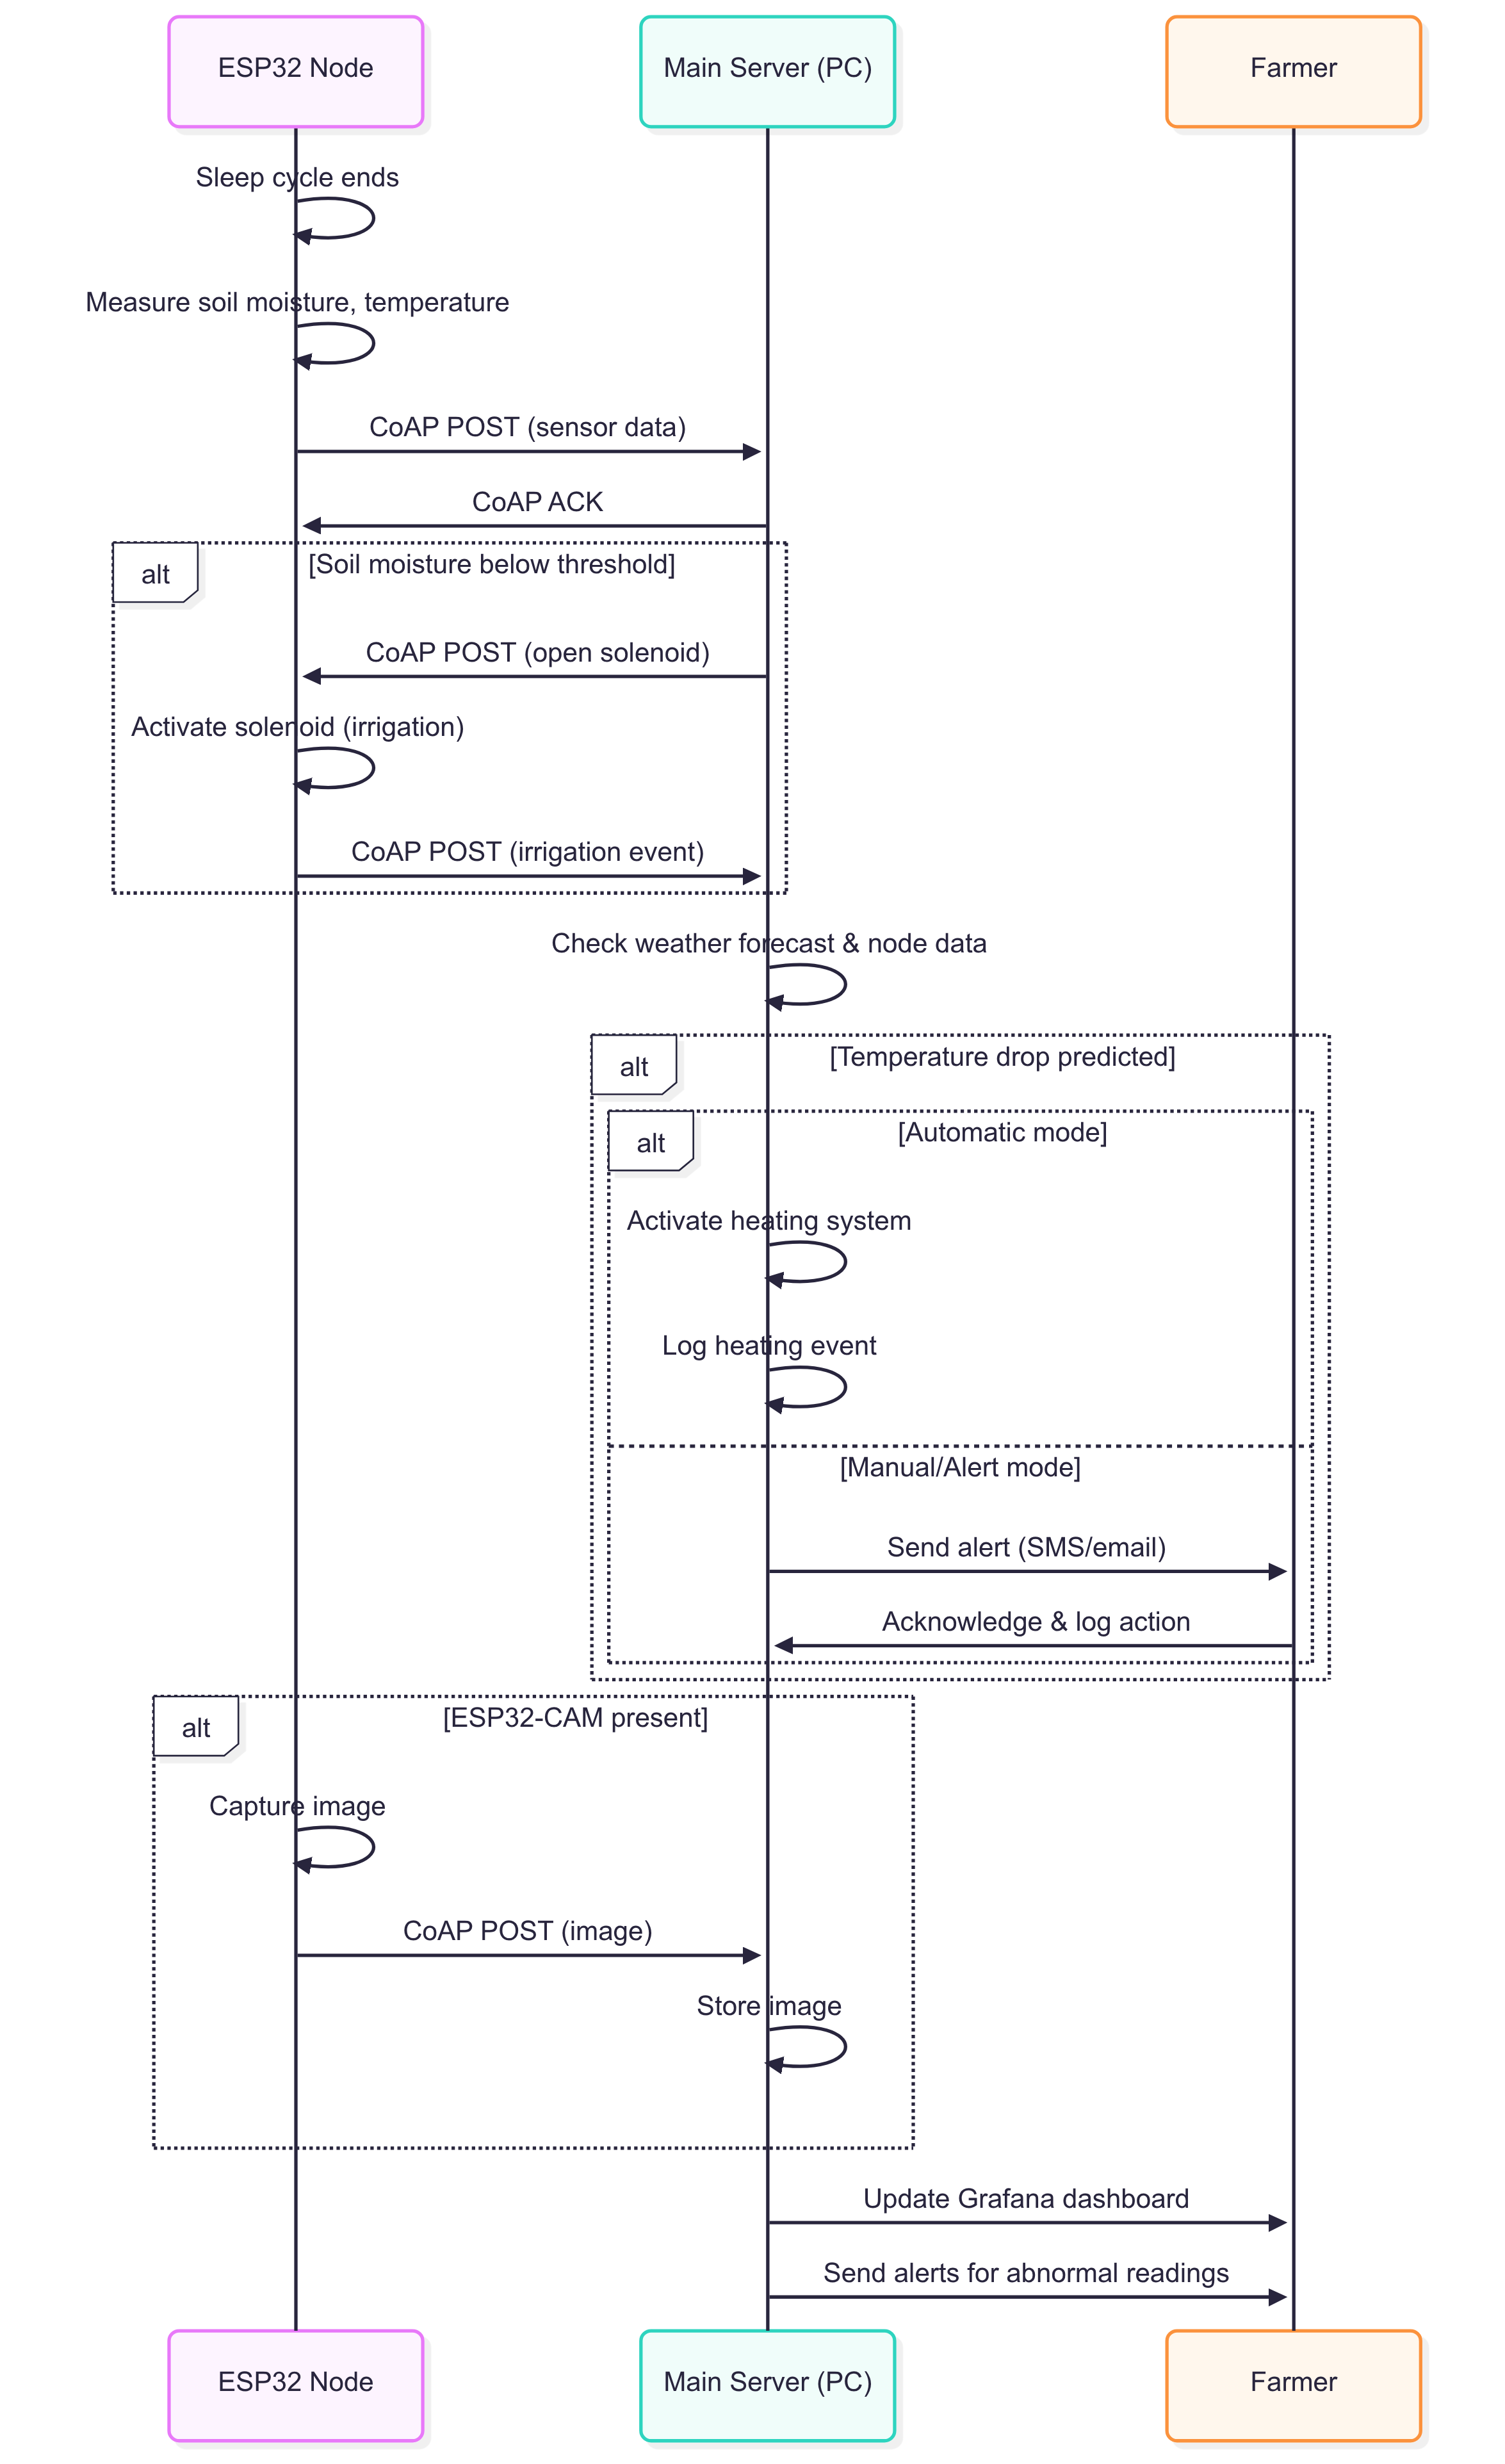
\includegraphics[width=0.85\textwidth]{images/nodeLifeCycleSequenceDiagram.png}
    \caption{Sequence diagram of the ESP32 node lifecycle: sleep, measurement, communication with the server, and irrigation control.}
    \label{fig:node-lifecycle}
\end{figure}

Figure~\ref{fig:node-lifecycle} illustrates the typical lifecycle of an ESP32 node in the greenhouse system. Each node periodically wakes from deep sleep, collects sensor data, transmits it to the server, and actuates the solenoid if required. This cycle is optimized for energy efficiency and reliable operation.

\paragraph{Flexible Irrigation System}
The water dripping system is modular and scalable. PVC tubes can be extended, and new nodes added wirelessly. The only constraint is maintaining adequate water pressure for uniform irrigation.

\subsection{Sample Sensor Data}
A typical 24-hour data sample includes temperature, humidity, light, soil moisture, and EC readings, demonstrating the system’s ability to capture key environmental metrics.
\begin{table}[H]
    \centering
    \begin{tabular}{|c|c|c|c|c|c|}
        \hline
        Time & Temp (\textdegree C) & Humidity (\%) & Light (lux) & Soil Moisture (\%) & EC (mS/cm) \\
        \hline
        00:00 & 22.1 & 65 & 0 & 45 & 1.2 \\
        06:00 & 20.5 & 70 & 100 & 48 & 1.1 \\
        12:00 & 28.3 & 55 & 12000 & 40 & 1.3 \\
        18:00 & 25.0 & 60 & 5000 & 42 & 1.2 \\
        \hline
    \end{tabular}
    \caption{Sample sensor data from a greenhouse node}
    \label{tab:sensordata}
\end{table}


\section{Communication Protocols}
RESTful CoAP is used for efficient, low-power communication between nodes and the server. The server manages data aggregation, storage, and control actions, ensuring reliable operation with less than 2\% packet loss and over 99.5\% uptime in tests.


\section{Data Collection and Visualization}
Sensor data is transmitted in real time (every 60 seconds or on significant change) via CoAP and stored in InfluxDB, a time-series database. An analytics pipeline processes soil moisture, EC, and environmental metrics, exposing real-time insights through FastAPI endpoints. Grafana dashboards provide live visualization and alerting, enabling prompt responses to changing soil conditions.

\subsection{Real-Time Soil Analysis and Node Mobility}
The system supports real-time analysis of soil parameters including moisture and EC, applying moving average filters for trend detection and anomaly alerts. Sensor nodes can be easily relocated across the greenhouse for spatial soil mapping. Upon relocation, nodes automatically reconnect via Wi-Fi, register with the CoAP server, and join the mesh network, enabling flexible coverage without manual setup.


\subsection{Use Case and Deployment}
The main actors are the farmer and the system administrator. Sensor nodes can be repositioned on-demand to focus measurements on critical zones and dynamically register with the CoAP server for immediate data collection and analysis.

\begin{figure}[H]
    \centering
    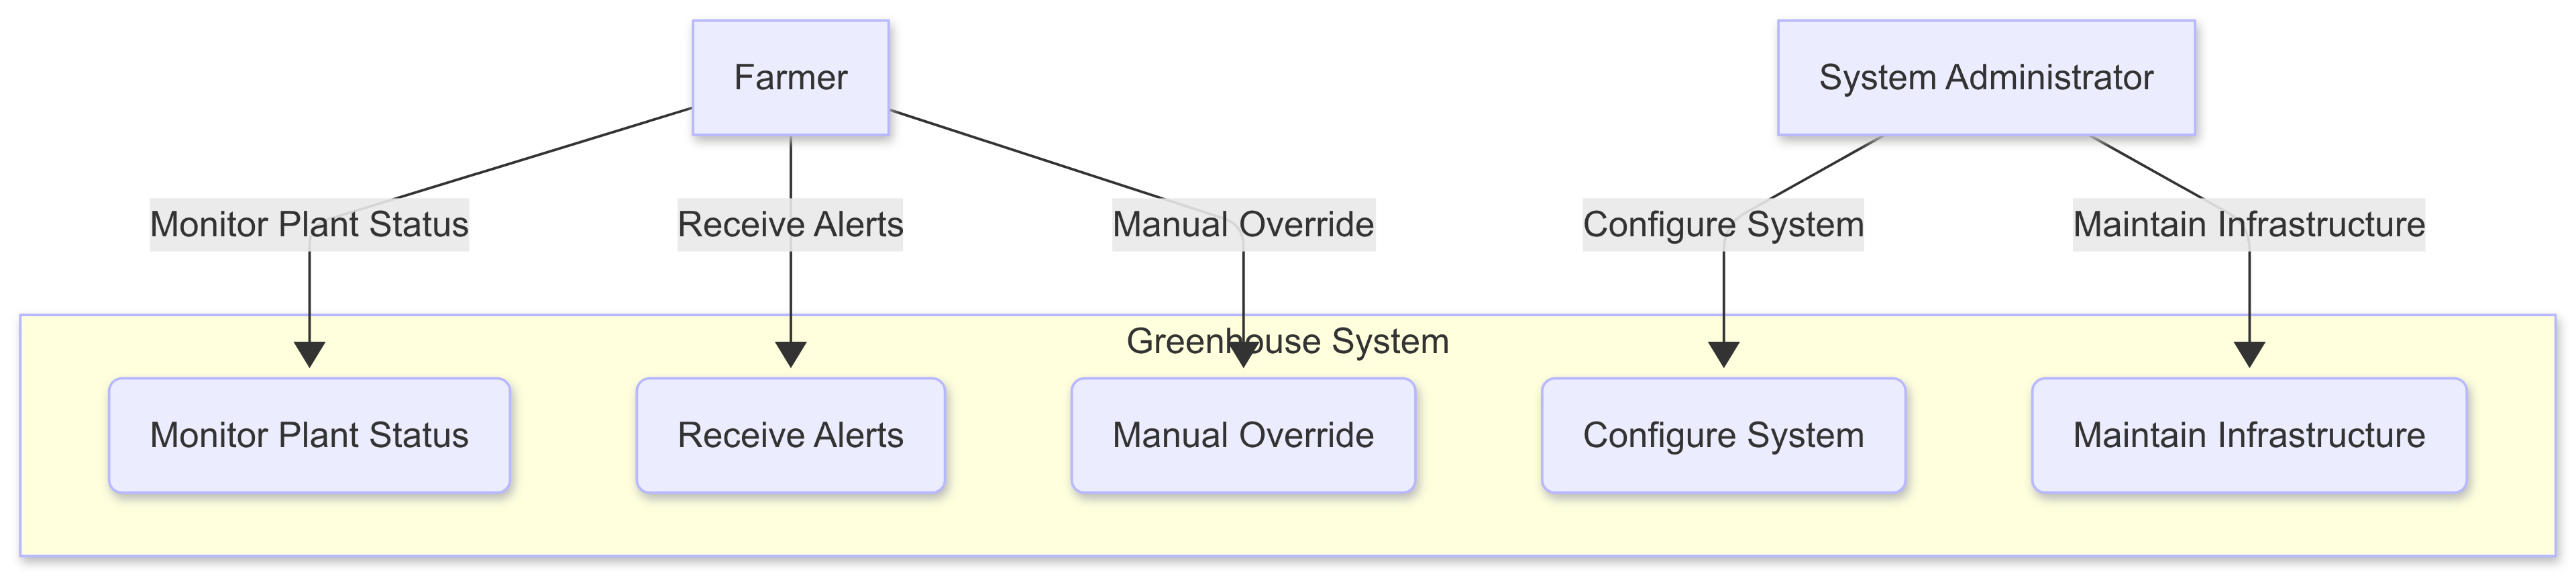
\includegraphics[width=0.7\textwidth]{images/useCaseDiagram.png}
    \caption{Use case diagram for the greenhouse system}
    \label{fig:usecase}
\end{figure}

Sensor nodes are deployed throughout the greenhouse, communicating via Wi-Fi to a local server. The server is connected to the internet for remote access and data backup. The deployment ensures scalability and reliability for large-scale greenhouse operations.

\begin{figure}[H]
    \centering
    \includegraphics[width=0.7\textwidth]{DeploymentDiagram.png}
    \caption{Deployment diagram of the greenhouse system}
    \label{fig:deployment}
\end{figure}

\subsection{Implementation Details}
The system was implemented in a 100 m$^2$ greenhouse with 50 mobile sensor nodes. Nodes were moved across 9 zones to perform spatial soil mapping, collecting over 5,000 real-time data points in 7 days. Each node maintained over 99% uptime, and the real-time analytics pipeline detected soil moisture trends within a 5% error margin. Each node was powered by a 2600mAh battery, providing up to 3 months of operation per charge. The server infrastructure included FastAPI, InfluxDB, and Grafana for data ingestion, analytics, and visualization.


\section{Control and Automation}
The server automates irrigation, temperature control, and alerting. It uses analytics to optimize resource use and can operate in fully automatic or manual/alert modes, allowing for both autonomous operation and farmer intervention.

Automation and analytics are key trends in smart agriculture~\cite{SmartAgReview,IoTGreenhouse2022}.

\subsection{Heating Control}
The system monitors temperature and weather forecasts, activating heating elements automatically or alerting the farmer as needed. All events are logged for transparency and analysis.

\textbf{Automatic Heating:}
\begin{itemize}
    \item If the forecast or measured temperature is predicted to fall below a set threshold (e.g., 15$^\circ$C), the server automatically activates heating elements (e.g., electric heater, water barrel circulation, or compost heat) if available.
    \item The system logs all heating events and their duration.
    \item If the system is in fully automatic mode, no notification is sent unless a fault is detected (e.g., heater failure, temperature not rising as expected).
\end{itemize}

\textbf{Manual/Alert Mode:}
\begin{itemize}
    \item If the system is set to manual or alert mode, the server sends an alert (SMS/email) to the farmer when a temperature drop is foreseen or detected, recommending manual intervention (e.g., turning on a heater, covering plants).
    \item The farmer can acknowledge the alert and log the action taken via the dashboard.
    \item The system can be configured to switch between automatic and manual modes depending on farmer preference or available equipment.
\end{itemize}

This dual-mode logic ensures both resilience and flexibility, allowing the greenhouse to operate autonomously when possible, but also supporting farmer intervention when needed or preferred.

\subsection{Irrigation Algorithm}
Irrigation is based on soil moisture and weather data, ensuring plants receive optimal water while minimizing waste.

\subsection{Alerts and Notifications}
The system sends email alerts for abnormal readings and scheduled tasks, supporting proactive management.


\section{Security and Reliability}
Data is transmitted over encrypted channels (TLS), with token-based authentication and regular backups. The system is designed for high reliability, with no data loss observed during extended testing.

Security and reliability are critical for IoT systems in agriculture~\cite{IoTSecurity2020}.


\section{Results and Discussion}
Deployment in a 100 m$^2$ greenhouse with 50 nodes demonstrated robust performance, with batteries lasting up to 3 months and over 200,000 sensor readings collected in 60 days. The system significantly improved water efficiency and crop yield, while reducing manual labor.

Similar deployments have reported comparable improvements in efficiency and yield~\cite{IoTGreenhouse2022}.


\section{Conclusion}
The smart greenhouse system described here leverages IoT technologies to deliver real-time monitoring, automation, and decision support for sustainable agriculture. The modular, scalable design makes it adaptable to diverse greenhouse environments, with proven benefits in efficiency and yield.


\section{Future Work}
Planned enhancements include:
\begin{itemize}
    \item \textbf{AI-based Image Analysis:} Integrate on-node or server-side AI for early detection of plant diseases and pest infestations using ESP32-CAM images, tailored to local crops.
    \item \textbf{Energy Autonomy:} Optimize solar charging and battery management for year-round, maintenance-free operation, including adaptive sleep cycles and energy-aware scheduling.
    \item \textbf{Predictive Control:} Use weather forecasts and historical data to anticipate irrigation and heating needs, reducing water and energy use while protecting crops from extreme events.
    \item \textbf{Modular Expansion:} Develop plug-and-play modules for additional sensors (e.g., CO$_2$, pH, EC) and actuators, supporting both greenhouse and open-field deployments.
    \item \textbf{Farmer Decision Support:} Enhance dashboards with actionable recommendations, economic analysis (cost/yield), and integration with local market data to support planning and sales.
    \item \textbf{Community and Open Source:} Release hardware designs, firmware, and backend code as open source, and build a local community of users and contributors in Central Asia.
\end{itemize}
These directions aim to make the system more robust, affordable, and useful for real-world agricultural challenges in Uzbekistan and similar regions.

\newpage


\section{References}
% Stop page numbering for References
\pagenumbering{gobble}
\begin{thebibliography}{99}
\bibitem{FAO2017} Food and Agriculture Organization (FAO), "The future of food and agriculture: Trends and challenges," 2017. \url{https://www.fao.org/}
\bibitem{SmartAgReview} Wolfert, S., Ge, L., Verdouw, C., & Bogaardt, M.-J. (2017). "Big Data in Smart Farming – A review," Agricultural Systems, 153, 69-80.
\bibitem{ESP32Survey} S. S. Kumar et al., "A Survey on ESP32: The New Microcontroller for IoT Applications," International Journal of Engineering Research & Technology, 2021.
\bibitem{CoAPRFC} Shelby, Z., Hartke, K., & Bormann, C. (2014). "The Constrained Application Protocol (CoAP)," RFC 7252. \url{https://coap.technology/}
\bibitem{Netafim2020} Netafim, "Smart Irrigation Solutions," 2020. \url{https://www.netafim.com/}
\bibitem{Priva2021} Priva, "Climate and Process Control for Greenhouses," 2021. \url{https://www.priva.com/}
\bibitem{IoTGreenhouse2022} Li, Y., Wang, N., Zhang, X., & Zhang, Y. (2022). "Design and Implementation of IoT-based Smart Greenhouse System," Computers and Electronics in Agriculture, 196, 106892.
\bibitem{InfluxDB2021} InfluxData, "InfluxDB Documentation," 2021. \url{https://www.influxdata.com/}
\bibitem{Grafana2021} Grafana Labs, "Grafana Documentation," 2021. \url{https://grafana.com/}
\bibitem{IoTSecurity2020} Sicari, S., Rizzardi, A., Grieco, L. A., & Coen-Porisini, A. (2020). "Security, privacy and trust in Internet of Things: The road ahead," Computer Networks, 76, 146-164.
\bibitem{Dataset to detect diseases in plant\'s leaf}.\url{https://www.kaggle.com/datasets/emmarex/plantdisease/data}

\end{thebibliography}

\end{document}
